\section{Extruding PLCL Results\label{results:extrudingPLCL}}

\subsection{Powder Extrusion Results\label{sec:results:extrudingPLCL:powderExtrusion}}
The output of the PLCL extrusion is shown below in~\autoref{fig:results:extrudingPLCL:powderExtrusion:filamentOutput}.

\begin{figure}[h!]
        \centering
        \includegraphics[width=\linewidth]{../figs/results/plclExtrusions/powderExtrusion/powder_filament_output.png}
        \caption{Extruder output of PLCL powder extrusion. Initial PLA output, transition from HDPE to PLCL (middle), and fully PLCL output (right).}
        \label{fig:results:extrudingPLCL:powderExtrusion:filamentOutput}
\end{figure}

The current output in $mA$ throughout this extrusion is shown below in~\autoref{fig:results:extrudingPLCL:powderExtrusion:currentOutput}. This was collected through DevoVision.

\begin{figure}[h!]
        \centering
        \includegraphics[width=0.7\linewidth]{../figs/results/plclExtrusions/powderExtrusion/powder_current_output.png}
        \caption{Current output throughout PLCL powder extrusion.}
        \label{fig:results:extrudingPLCL:powderExtrusion:currentOutput}
\end{figure}

Discussion of these results can be found in~\fullref{sec:discussion:extrudingPLCL:powderExtrusion}.

\subsection{Pellet Extrusions Results\label{results:extrudingPLCL:pelletExtrusions}}

\subsubsection{Initial Pellet Extrusion Results\label{sec:results:extrudingPLCL:pelletExtrusions:initialPelletExtrusion}}

No quantitative results of this extrusion were collected due to issues using DevoVision. Qualitatively, this extrusion resulted in variable output, clumping at the hopper, and an apparent separation of PLA and PCL pellets with PCL moving to the top of the hopper and PLA moving to the bottom.

Discussion of this extrusion can be found in~\fullref{sec:discussion:extrudingPLCL:pelletExtrusions:initialPelletExtrusion}.

\subsubsection{PCL Temperature Study Results\label{sec:results:extrudingPLCL:pelletExtrusions:pclTempStudy}}

Output from DevoVision is limited for this study because the version of DevoVision being used was outdated and did not support file downloading.

Qualitatively, the current began to rise above 6000 mA at roughly 70\textcelsius ~while lowering to 60\textcelsius. At 80\textcelsius ~the current began to lower and stabilize. This is shown below in Figure~\ref{fig:results:extrudingPLCL:pelletExtrusions:pclTempCurrentRise}

\begin{figure}[h!]
        \centering
        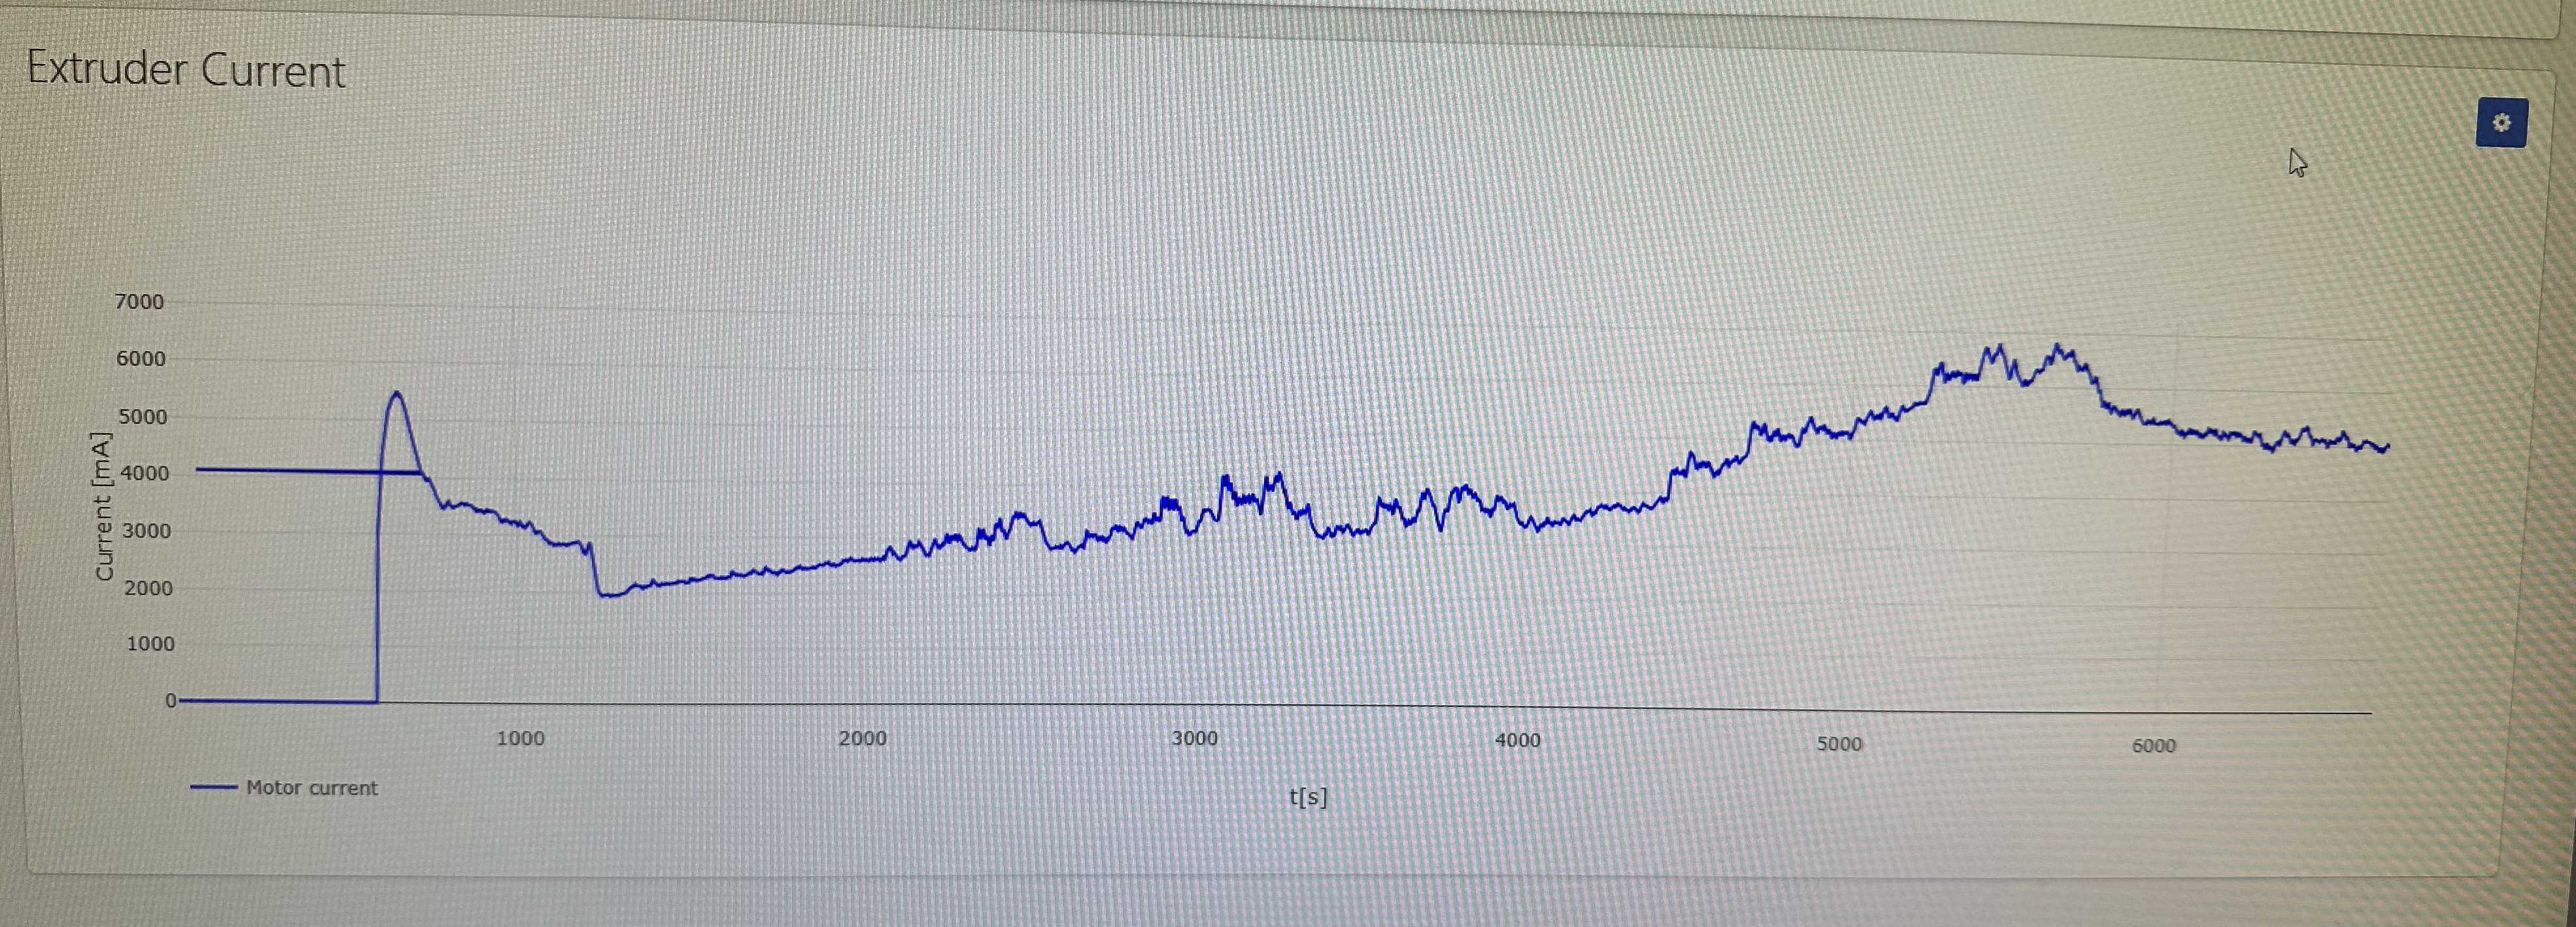
\includegraphics[width=\linewidth]{../figs/results/plclExtrusions/pelletExtrusions/pcl_temp_study_devovision_current_rise.png}
        \caption{Rise in current as heaters approached 60\textcelsius.}
        \label{fig:results:extrudingPLCL:pelletExtrusions:pclTempCurrentRise}
\end{figure}

Filament output was steady and of proper quality between 80\textcelsius ~and 150\textcelsius. Between 160\textcelsius ~and 180\textcelsius ~the PCL pellets were extrudable but began clogging more easily.

Discussion of these results can be found in ~\fullref{sec:discussion:extrudingPLCL:pelletExtrusions:pclTempStudy}.

\subsubsection{Manual Starve Feeding Results\label{sec:results:extrudingPLCL:pelletExtrusions:manualStarveFeeding}}

The results of the manual starve feeding from 80\textcelsius ~to 110\textcelsius ~are shown below in~\autoref{tab:results:extrudingPLCL:pelletExtrusions:manualStarveFeedingSummary}.

\begin{table}[h!]
        \centering
        \caption{Manual starve feeding pouring statistics by temperature.}
        \label{tab:results:extrudingPLCL:pelletExtrusions:manualStarveFeedingSummary}
        \begin{tabular}{c c c c c}
                \hline
                \textbf{Temperature (°C)} & \textbf{Avg Time Between Pours} & \textbf{Std Dev} & \textbf{Avg Amount Poured (mL)} & \textbf{Std Dev} \\
                \hline
                90                        & 0:01:59                         & 0:00:15          & 9.174                           & 3.421            \\
                100                       & 0:02:24                         & 0:00:26          & 9.978                           & 2.345            \\
                110                       & 0:02:24                         & 0:00:10          & 9.635                           & 1.237            \\
                \hline
                \textbf{Total}            & \textbf{0:02:16}                & \textbf{0:00:17} & \textbf{9.595}                  & \textbf{2.335}   \\
                \hline
        \end{tabular}
\end{table}

\subsubsection{Initial PLCL Extrusion with Starve Feeder Results\label{sec:results:extrudingPLCL:pelletExtrusions:initialStarveFeederExtrusion}}

In this initial PLA/PCL extrusion using a starve feeder, PLCL was successfully extruded between 180\textcelsius ~and 160\textcelsius ~in 5 degree increments. Filament output directly from the nozzle across this temperature range is shown below in Figure~\ref{fig:results:extrudingPLCL:pelletExtrusions:initialStarveFeederExtrusion:nozzleOutput}.

\begin{figure}[h!]
        \centering
        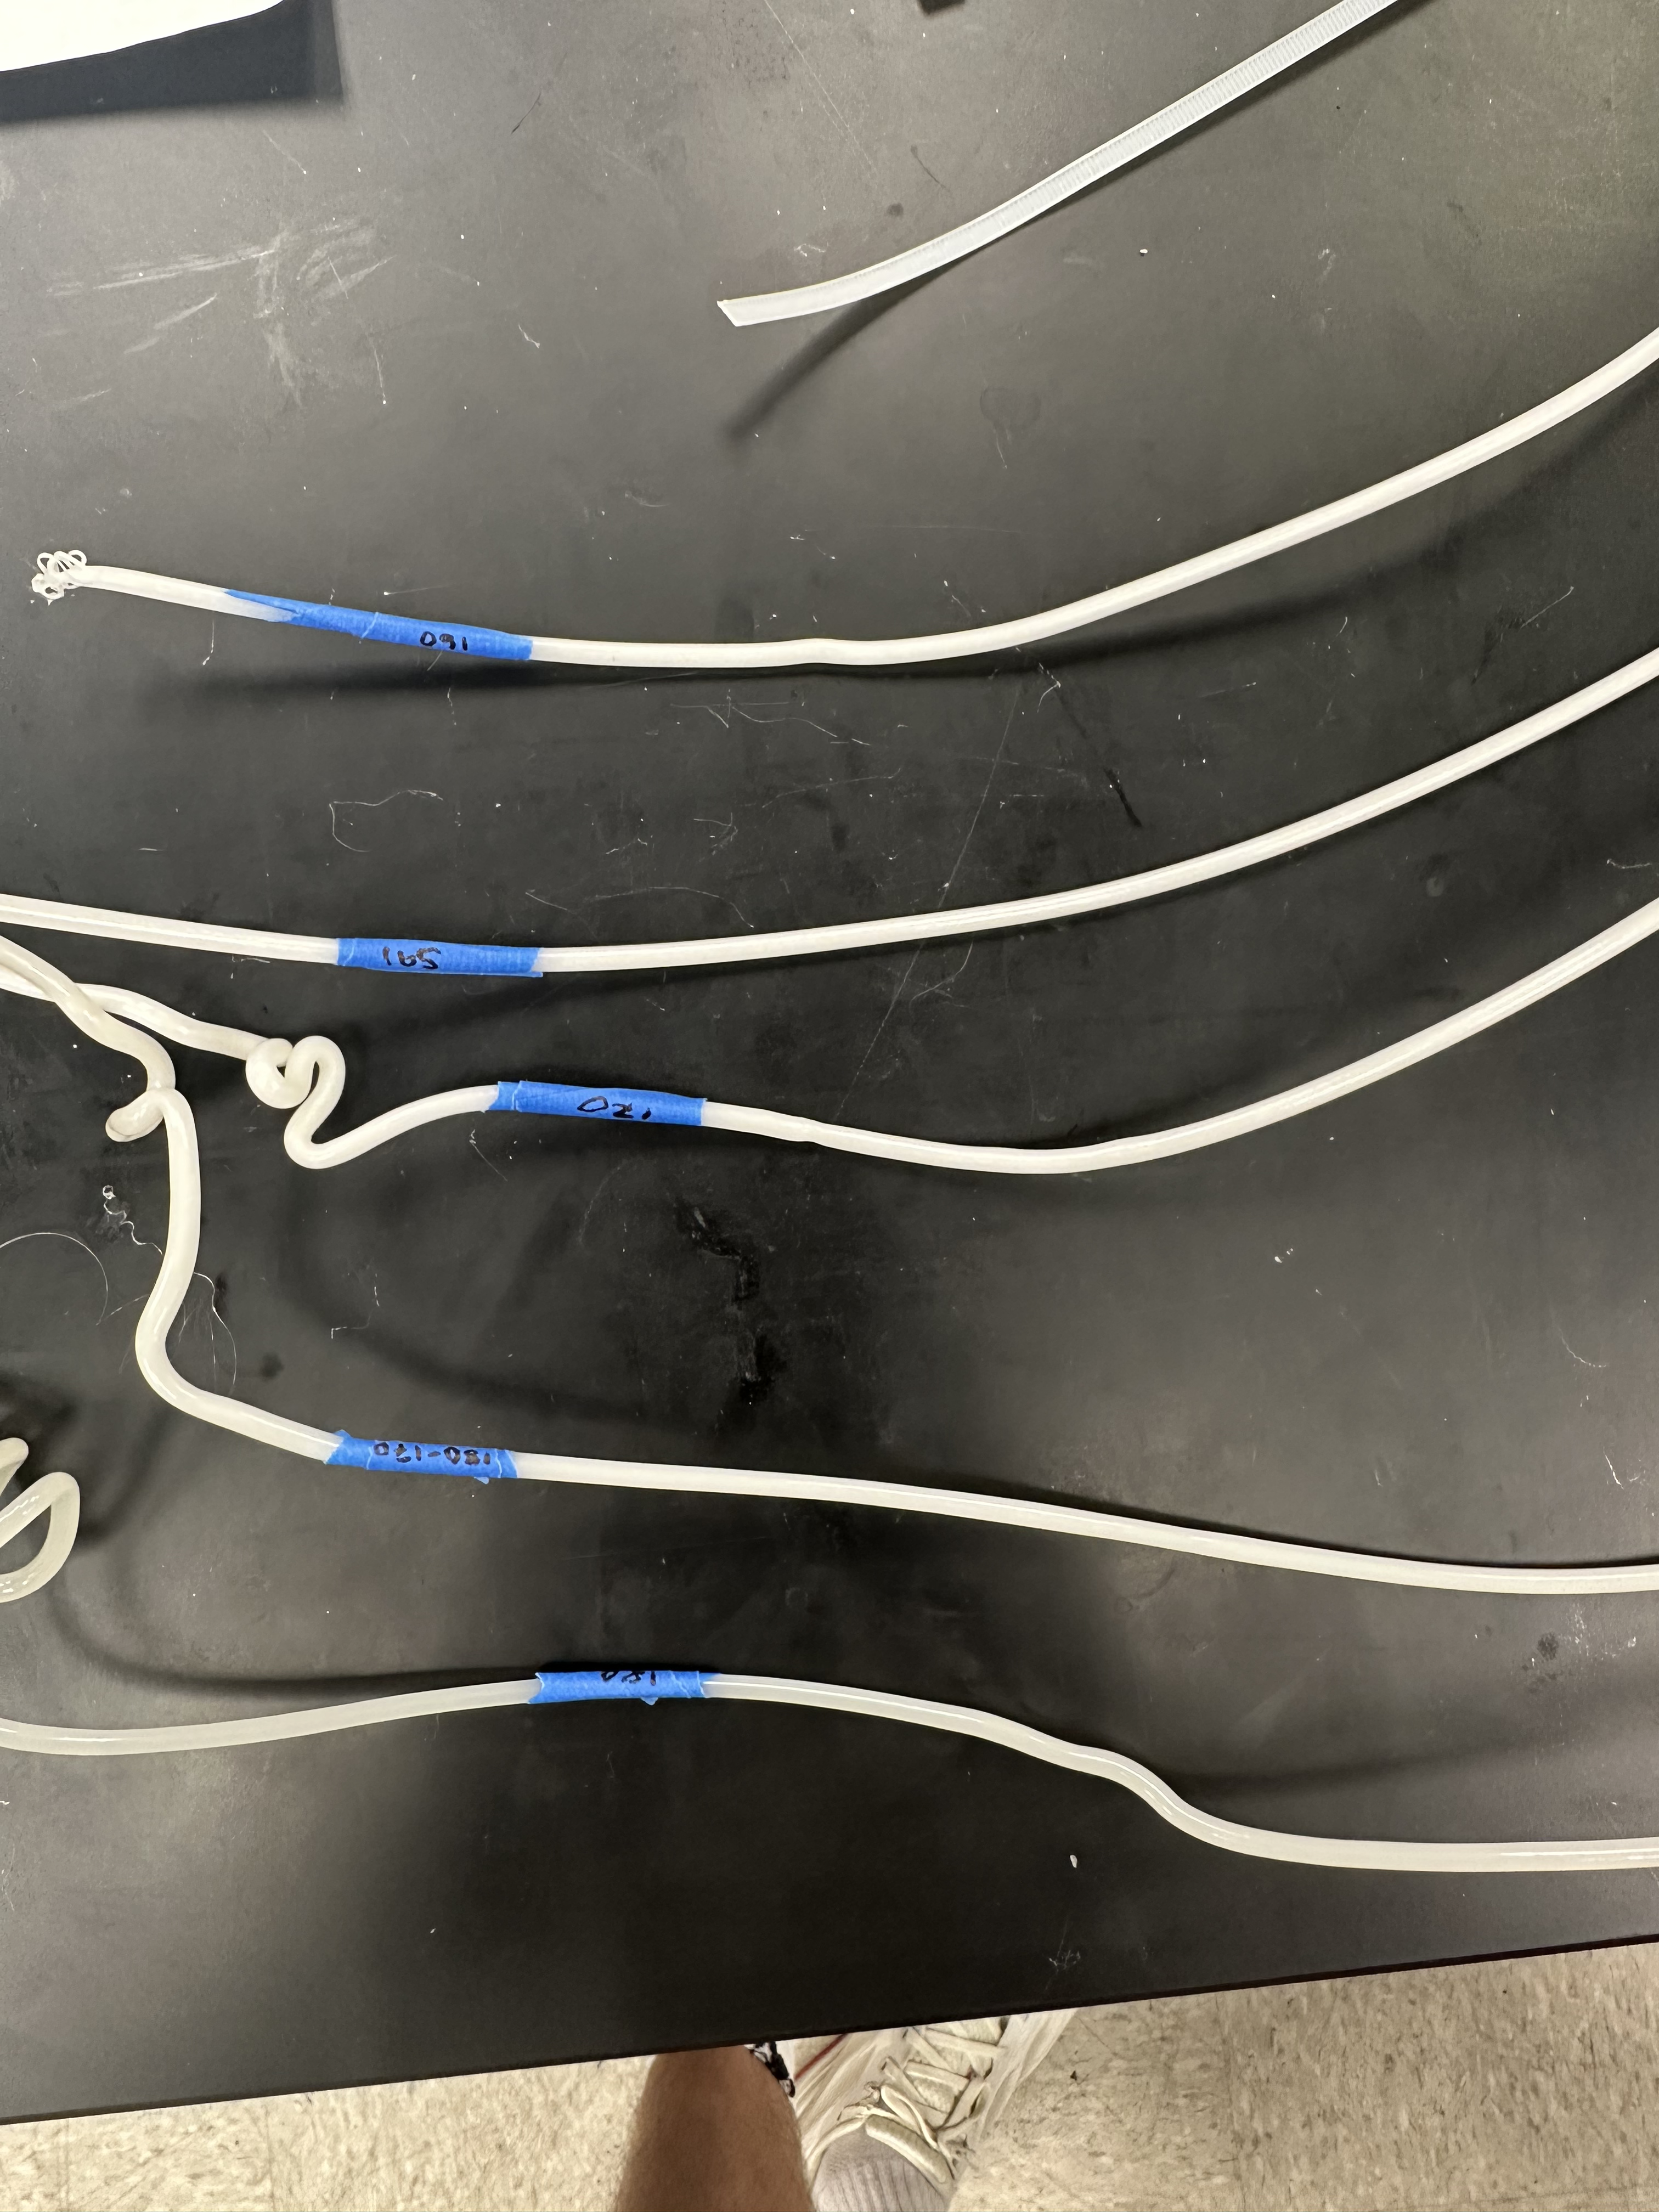
\includegraphics[width=0.5\linewidth]{../figs/results/plclExtrusions/pelletExtrusions/starveFeederExtrusions/starve_feeder_initial_plcl_extrusion_nozzle_output.png}
        \caption{Nozzle output of initial starve feeder based PLCL extrusion from 160\textcelsius (top) to 180\textcelsius ~(bottom).}
        \label{fig:results:extrudingPLCL:pelletExtrusions:initialStarveFeederExtrusion:nozzleOutput}
\end{figure}

Raw data of the extrusion was not saved due to an outdated version of DevoVision being used. However, when spooling, the thickness of the spooled filament was highly variable with an average thickness of 1.40mm. Adjustments to RPM and pellet dispenser pour rate did not improve the filament thickness average or variability.

Discussions of these results can be found in ~\fullref{sec:discussion:extrudingPLCL:pelletEtrusions:initialStarveFeederExtrusion}.

\subsubsection{Addressing Filament Thickness Results\label{sec:results:extrudingPLCL:pelletExtrusions:addressingFilamentThickness}}

\paragraph*{Adjusting Heat Zones}

Filament thickness resulting from turning heater 4 and then heaters 4 and 3 as low as they could go (100\textcelsius) are shown in Figure~\ref{fig:results:extrudingPLCL:pelletExtrusions:addressingFilamentThickness:h4Andh3Off}

\begin{figure}[h!]
        \centering
        \includegraphics[width=0.7\linewidth]{../figs/results/plclExtrusions/pelletExtrusions/starveFeederExtrusions/filament_thickness_turning_heater_off.png}
        \caption{Filament thickness after turning H4 and H3 to low.}
        \label{fig:results:extrudingPLCL:pelletExtrusions:addressingFilamentThickness:h4Andh3Off}
\end{figure}

\paragraph*{Extruding PLCL Regrind}

Data logging of the extruded PLCL regrind could not be recorded due to software issues with DevoVision. However, while it extruded from the nozzle thicker than the first pass of PLCL, the filament thickness while spooling was still too thin. Figure~\ref{fig:results:extrudingPLCL:pelletExtrusions:addressingFilamentThickness:regrindOutput} shows the initial output from the nozzle when extruding PLCL regrind.

\begin{figure}[h!]
        \centering
        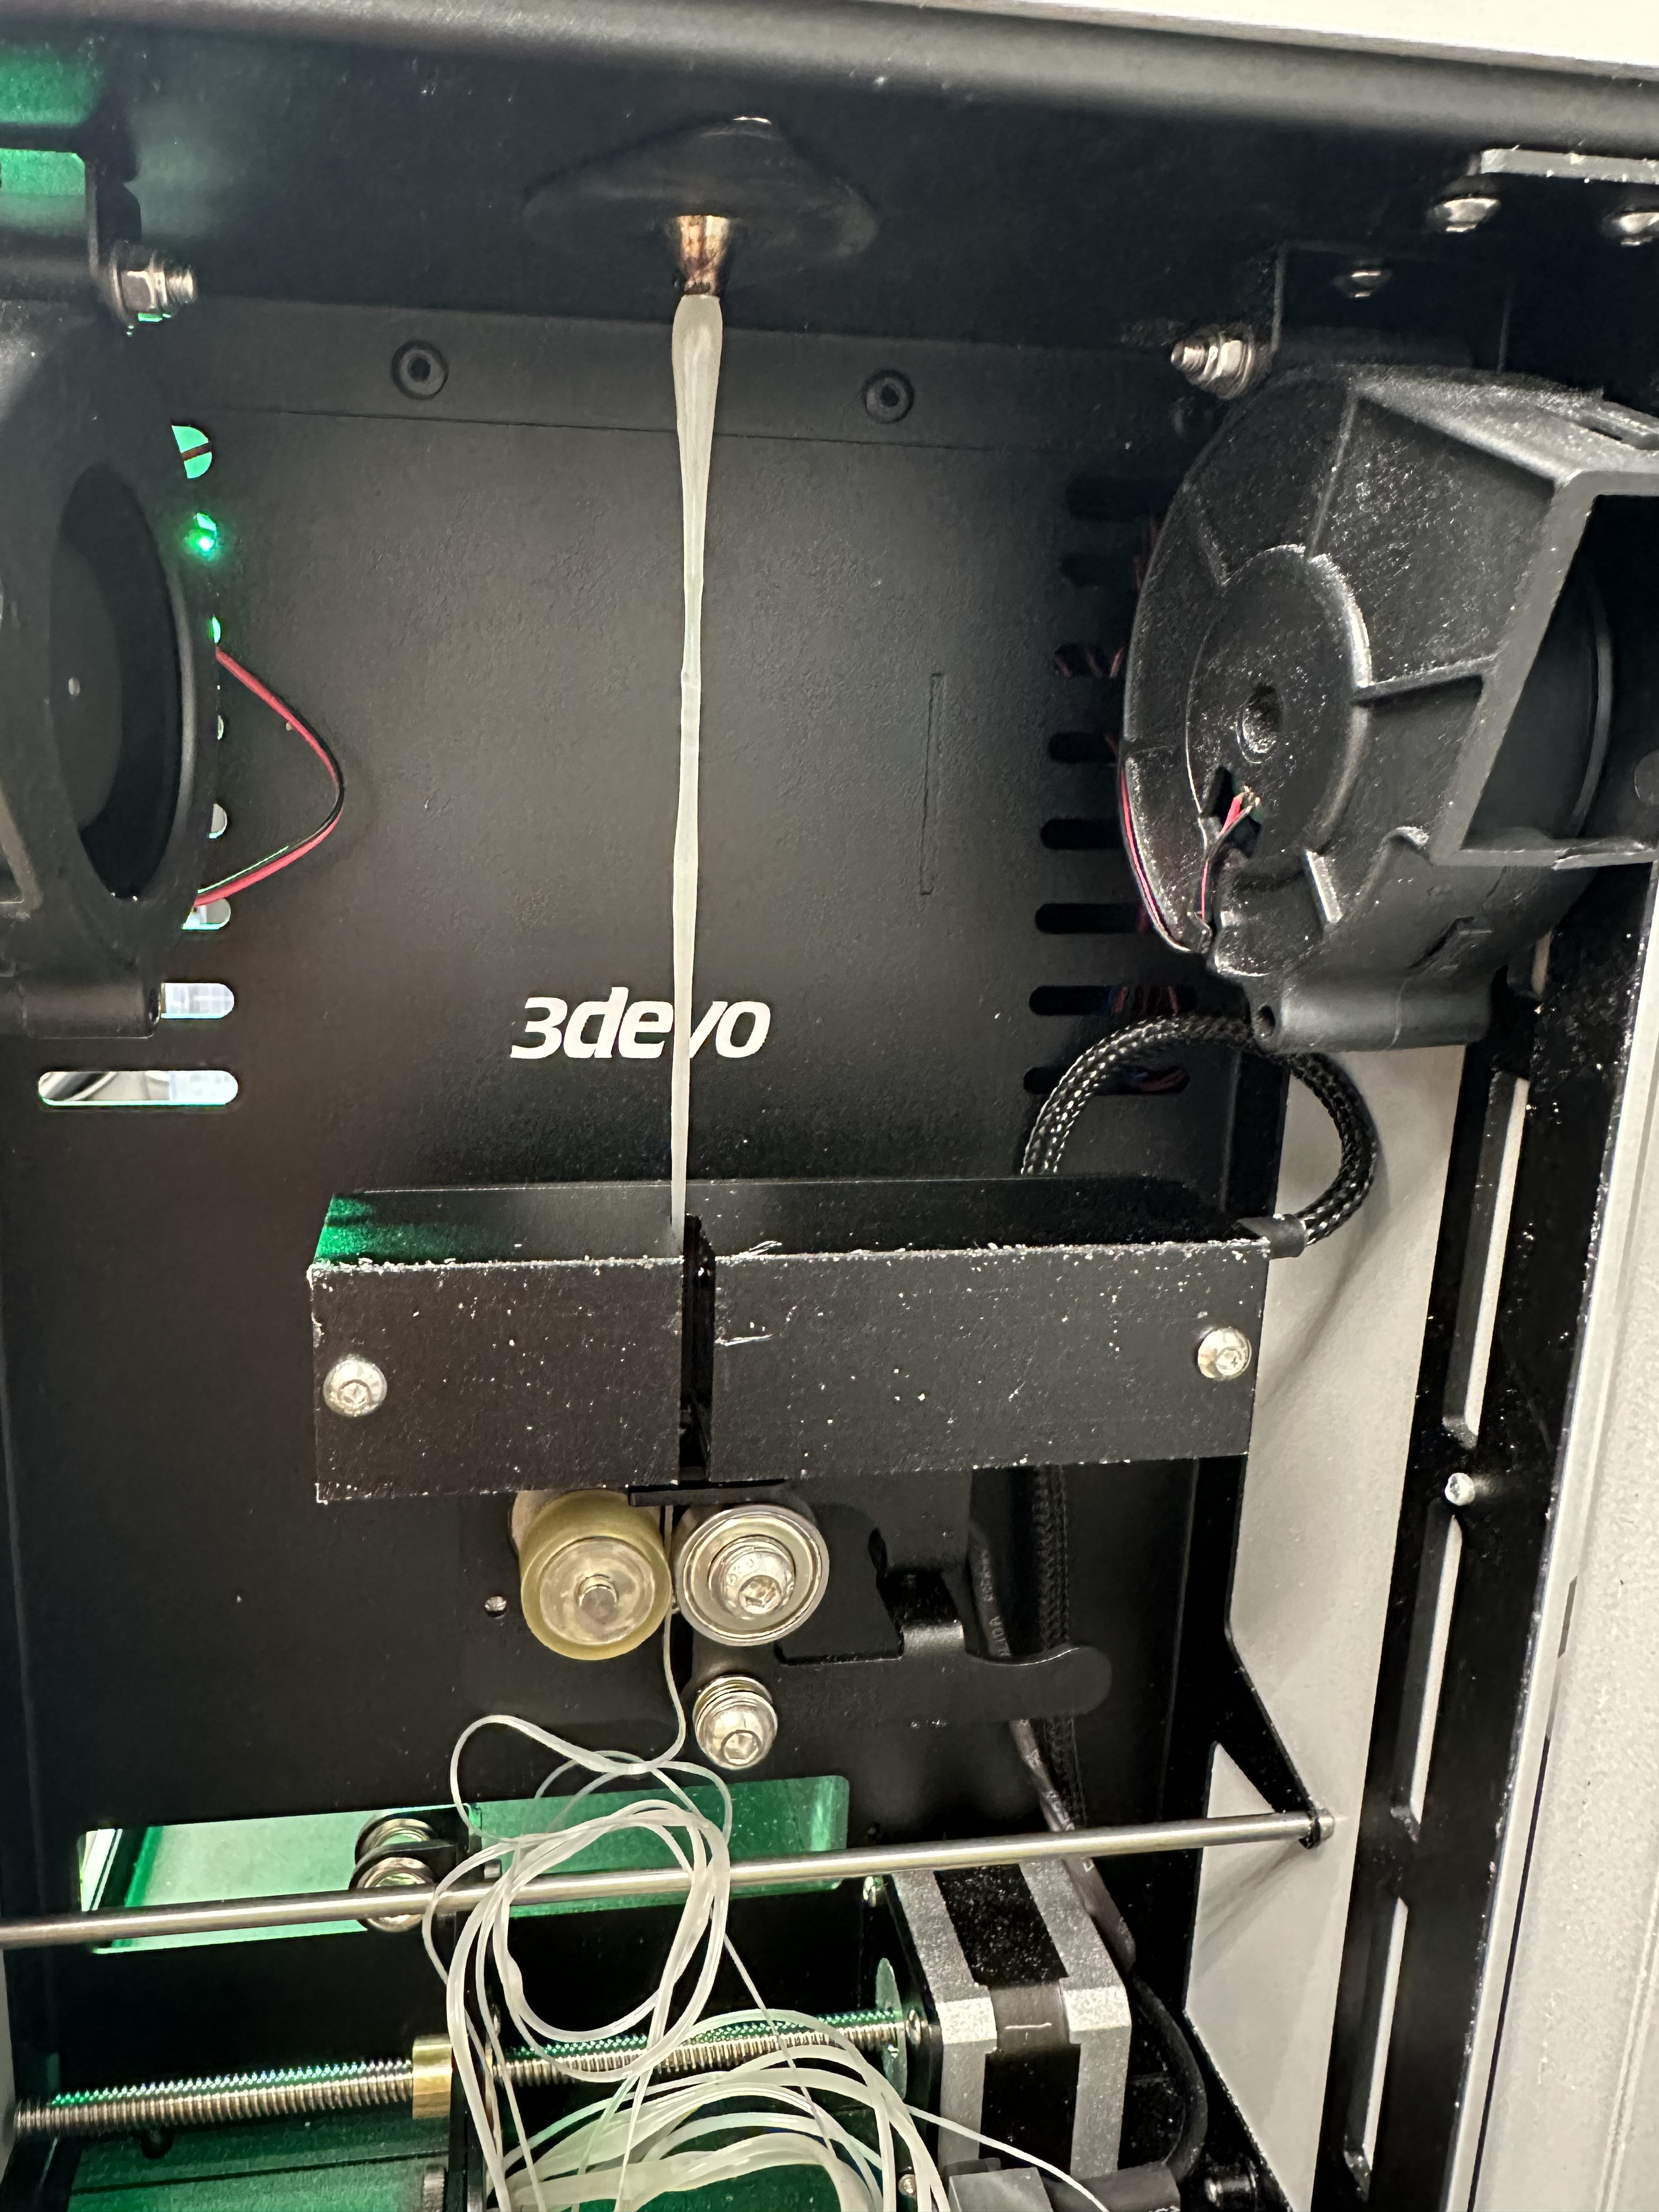
\includegraphics[width=0.5\linewidth]{../figs/results/plclExtrusions/pelletExtrusions/starveFeederExtrusions/plcl_regrind_extrusion_output.png}
        \caption{Initial output of PLCL regrind from the nozzle.}
        \label{fig:results:extrudingPLCL:pelletExtrusions:addressingFilamentThickness:regrindOutput}
\end{figure}

Discussion of these results can be found in ~\fullref{sec:discussion:extrudingPLCL:pelletExtrusions:addressingFilamentThickness}.

\subsection{Felfil Evo Results\label{sec:results:extrudingPLCL:pelletExtrusions:felfilEvo}}

\subsubsection{Initial PLCL Extrusion Results\label{sec:results:extrudingPLCL:pelletExtrusions:felfilEvo:initialPLCL}}

\paragraph*{Filament Quality}
The Felfil Evo was able to properly extrude good-quality PLCL filament as shown in Figure~\ref{fig:results:extrudingPLCL:felfilEvo:initialPLCL}

\begin{figure}[h!]
        \centering
        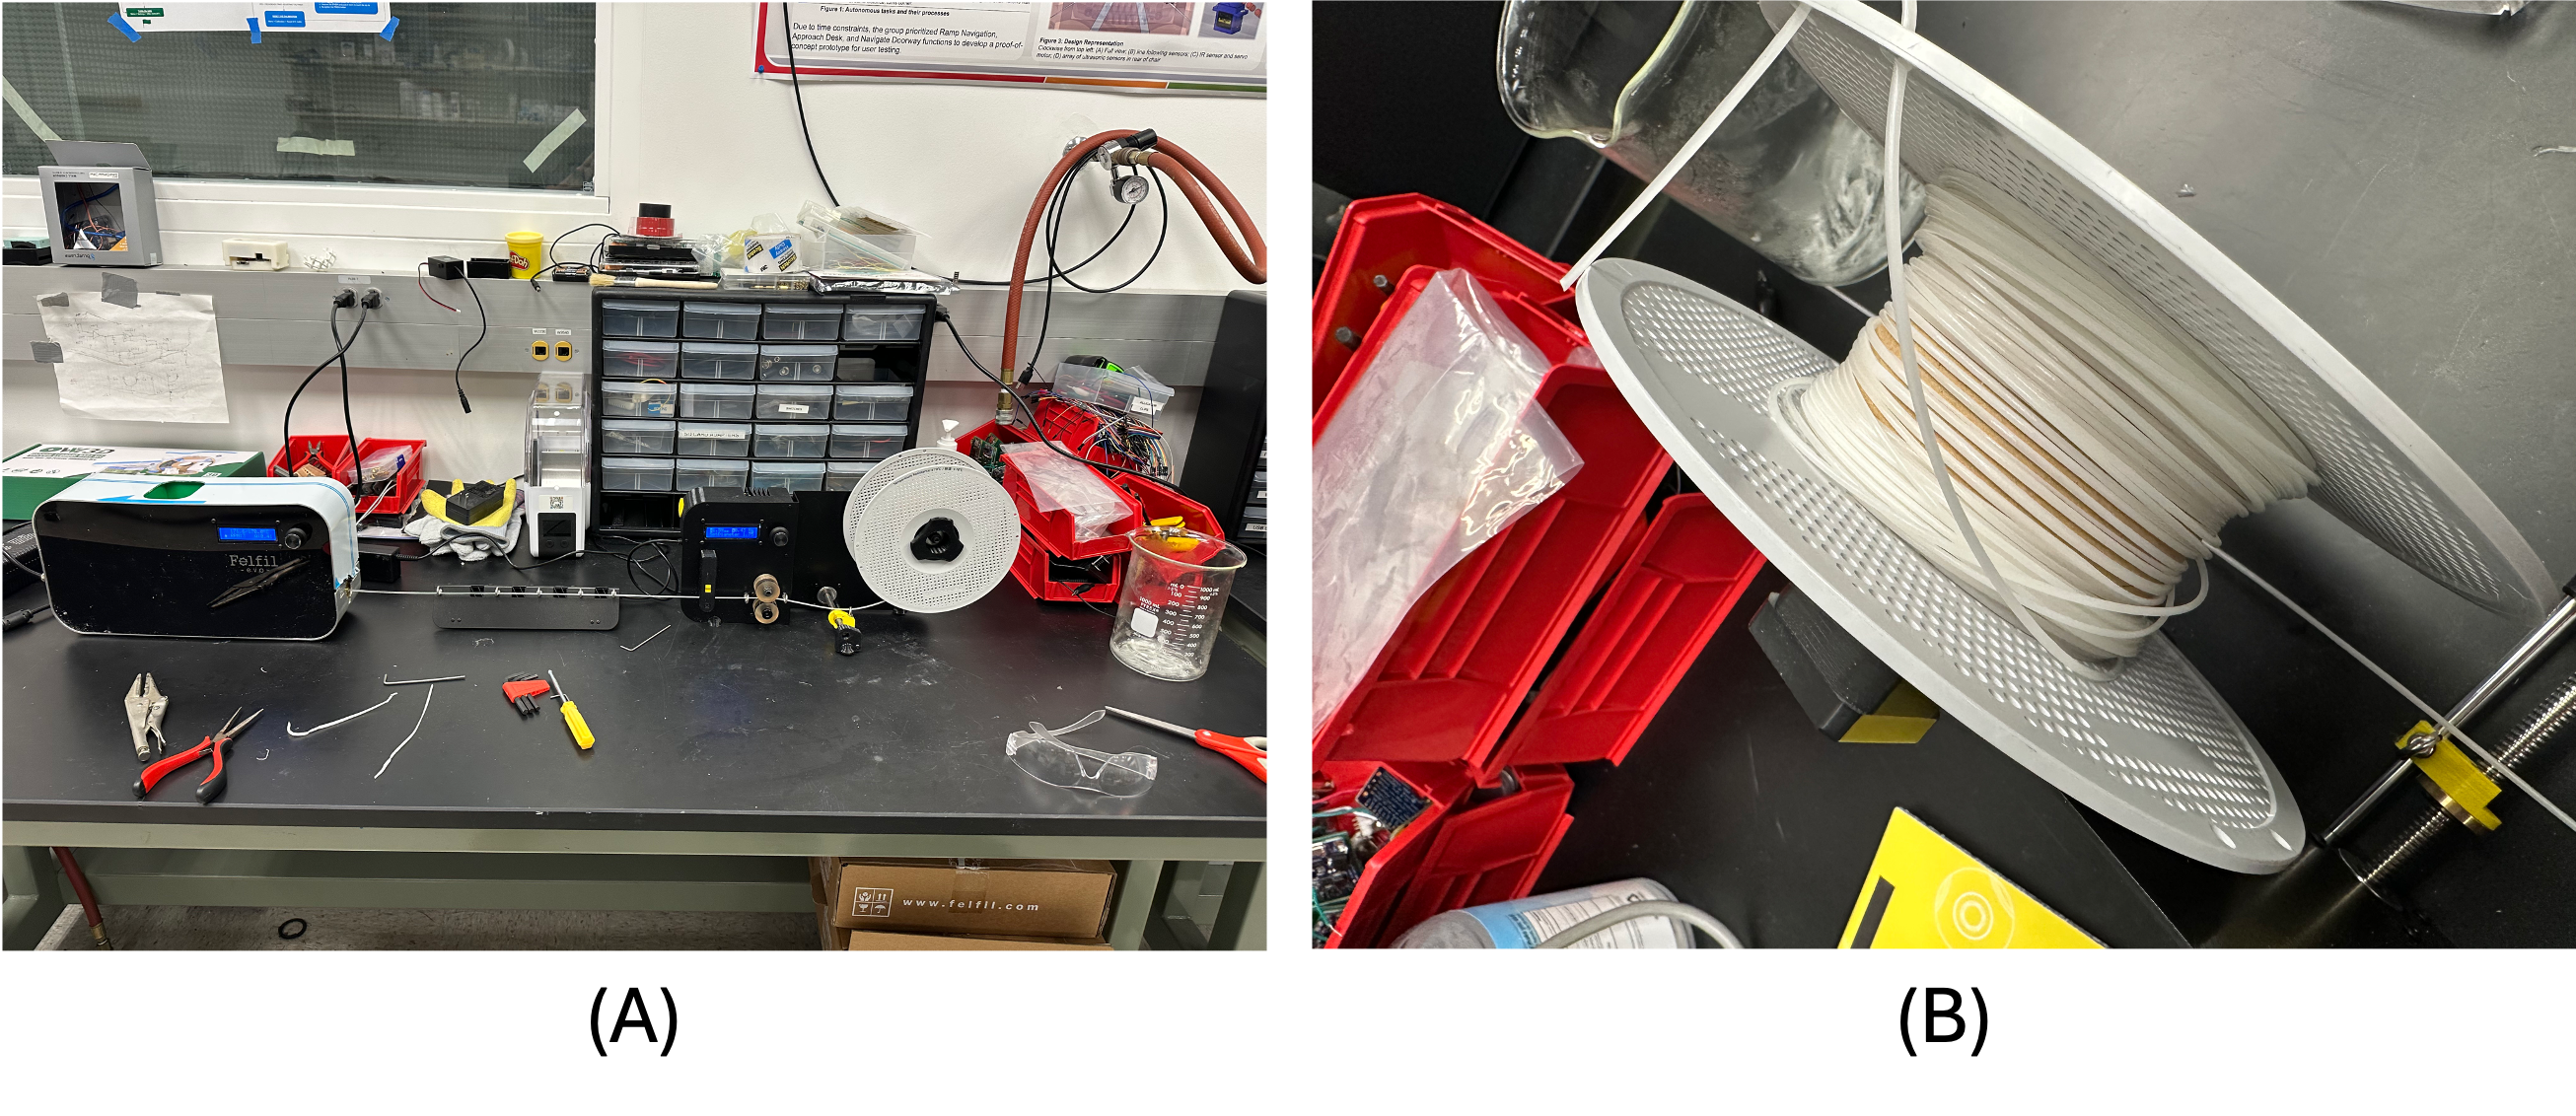
\includegraphics[width=\linewidth]{../figs/results/plclExtrusions/pelletExtrusions/felfilEvo/initial_plcl_extrusion.png}
        \caption{Initial PLCL extrusion with Felfil Evo. Extrusion setup (A) and output filament (B).}
        \label{fig:results:extrudingPLCL:felfilEvo:initialPLCL}
\end{figure}

\paragraph*{Filament Thickness}

\subsection{Purging Extruder Results\label{sec:results:extrudingPLCL:pelletExtrusions:purgingExtruder}}

\subsubsection{Initial Purging Process Results\label{sec:results:extrudingPLCL:pelletExtrusions:purgingExtruder:initialPurge}}

The initial output from the DevoClean MT purge is shown below in Figure~\ref{fig:results:extrudingPLCL:initialMTPurgeIndividual} and Figure~\ref{fig:results:extrudingPLCL:initialMTPurgeOverview}

\begin{figure}[h!]
        \centering
        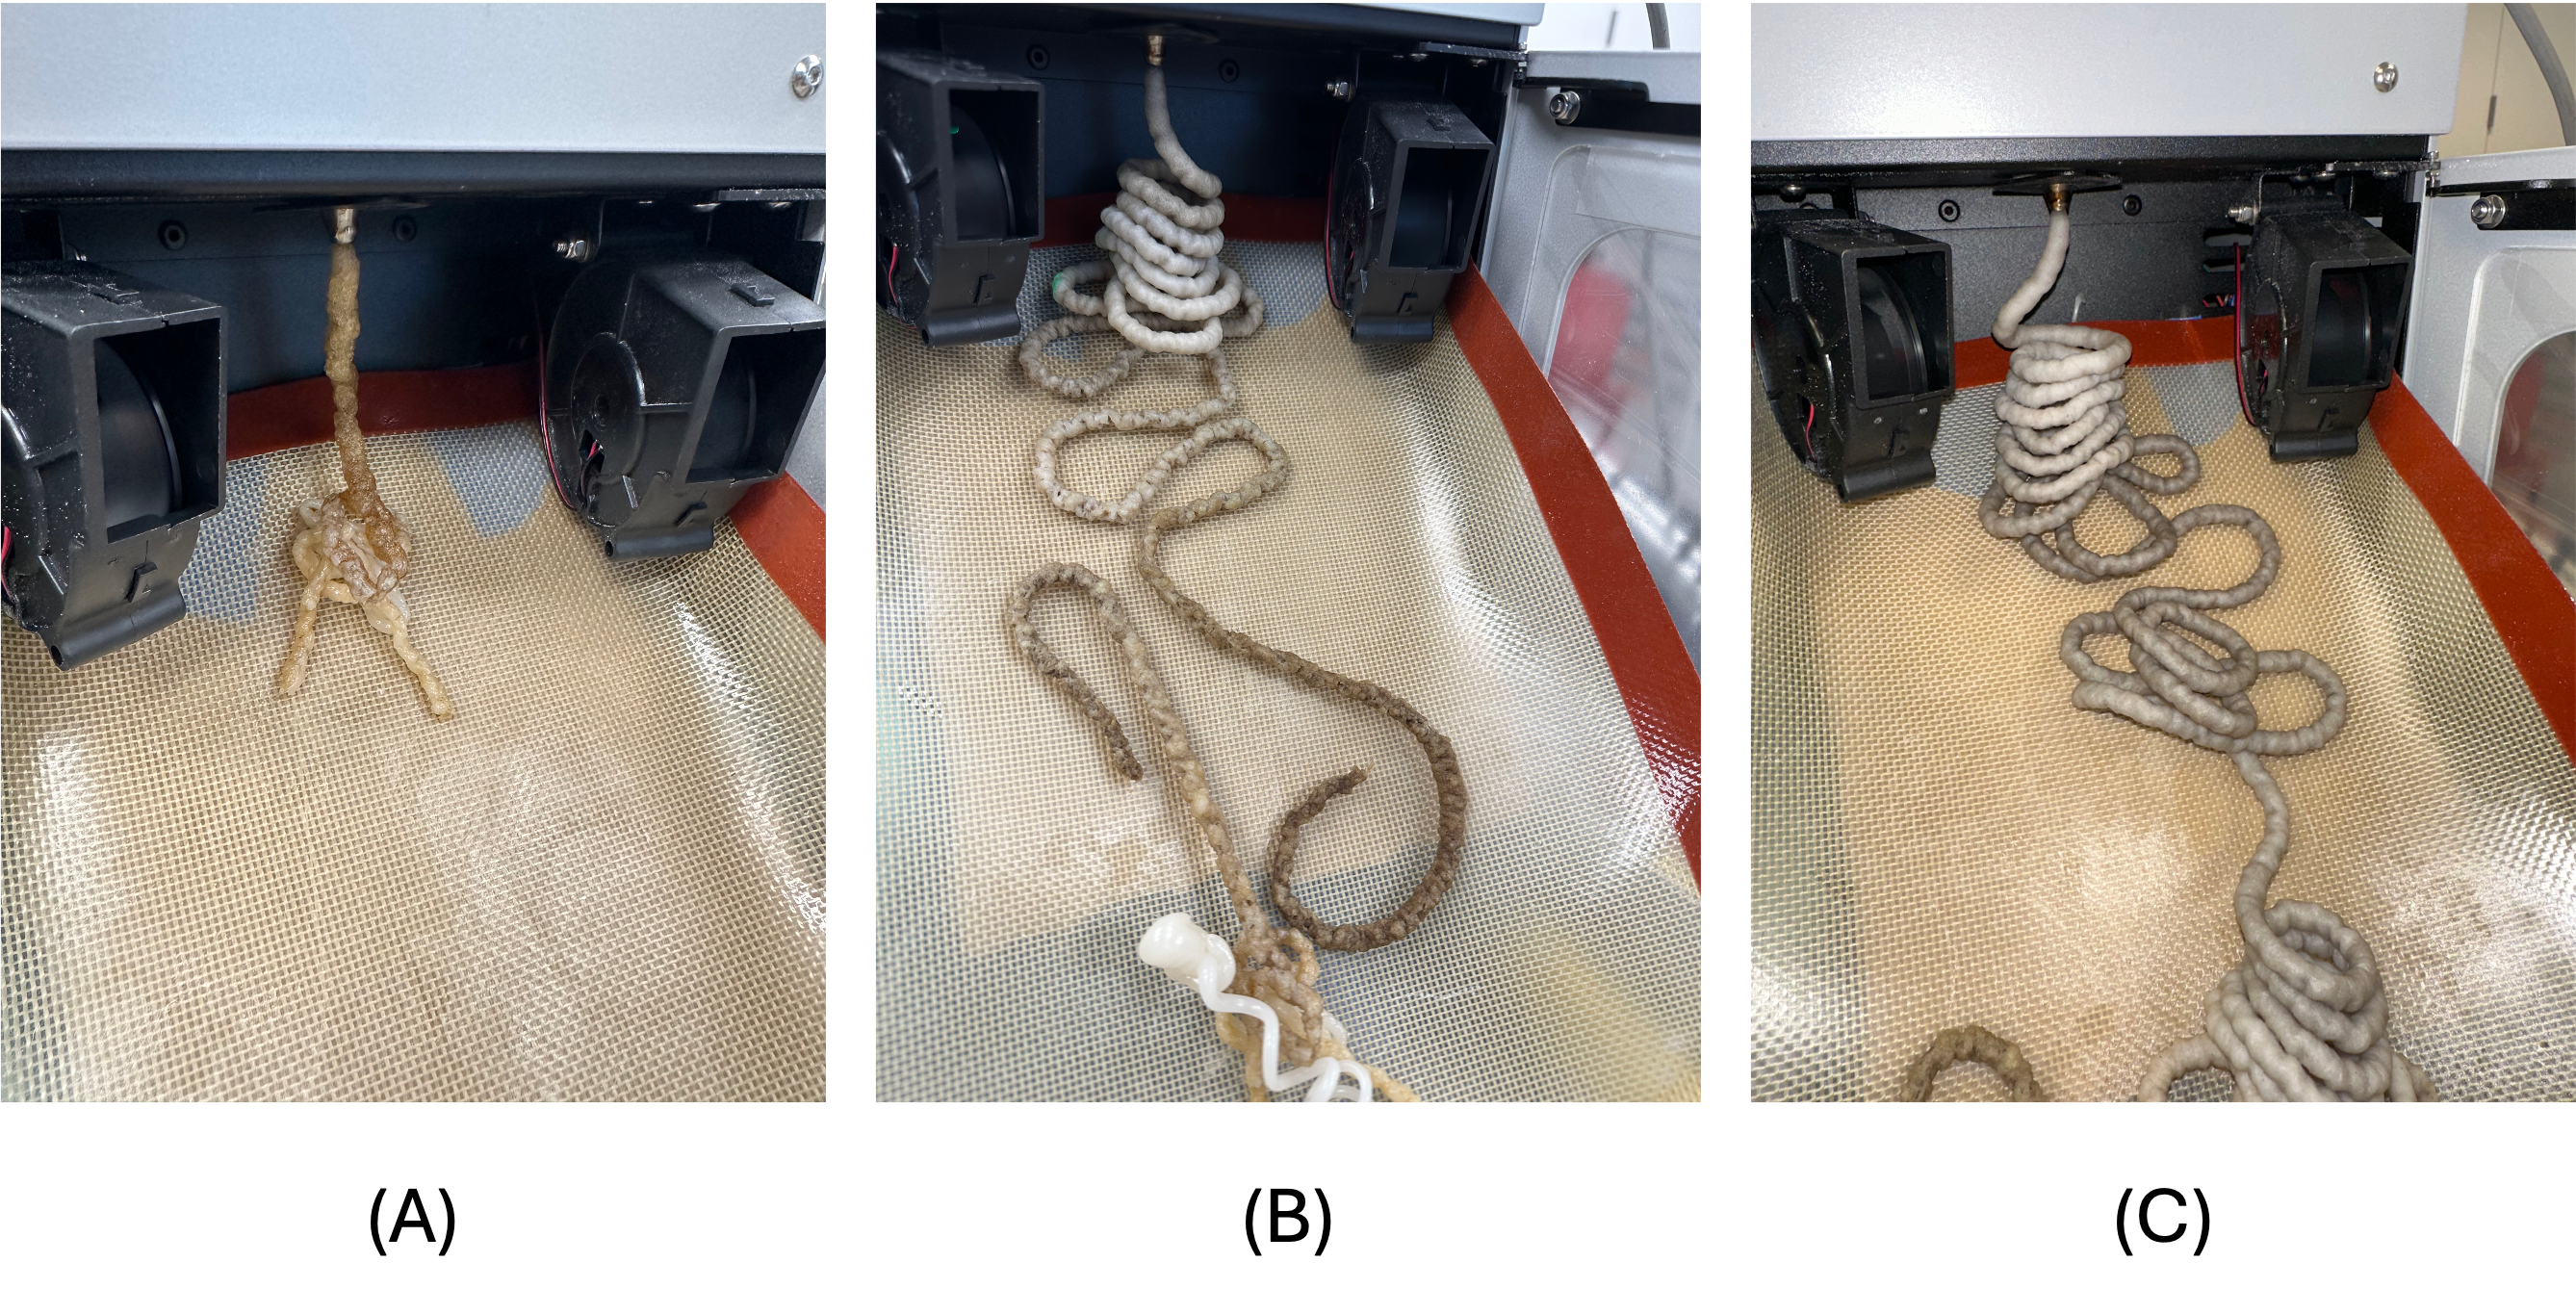
\includegraphics[width=0.7\linewidth]{../figs/results/plclExtrusions/purgingExtruder/devoclean_mt_puge_output.png}
        \caption{Initial DevoClean MT Purge. Contaminated output (A) transitioning to cleaner output (B) and finally to fully clean output (C).}
        \label{fig:results:extrudingPLCL:initialMTPurgeIndividual}
\end{figure}

\begin{figure}[h!]
        \centering
        \includegraphics[width=0.7\linewidth]{../figs/results/plclExtrusions/purgingExtruder/devoclean_mt_puge_output_overview.png}
        \caption{Overview of DevoClean MT purging process. Initial contaminants (bottom) to clean output (top).}
        \label{fig:results:extrudingPLCL:initialMTPurgeOverview}
\end{figure}

Discussion of these results can be found in {sec:discussion:extrudingPLCL:pelletExtrusions:purgingExtruder:initialPurge}
